\section{Discusión}

Una vez que se han conseguido los resultados correspondientes, se procede a discutir los diferentes problemas y hallazgos en esta sección

\subsection{Análisis inicial de genes y proteínas}

\subsubsection{Red PPI SARS-Cov2}

La red de interacción entre proteínas del SARS-Cov2 se compone de un total de \emph{332 proteínas cebo del virus que interactúan con el organismo humano}. Una proteína cebo es aquella que se usa para identificar las interacciones de las otras proteínas que nos interesa analizar (conocidas como \textit{proteínas cebo}). Suelen ser elegidas aquellas de las que se dispone información 

\newline

La red mostrada a continuación muestra un esquema de colores que identifican aquellas proteínas que participan en una misma interacción viral. En la figura se muestran las 10 proteínas con mayor interacción entre ellas así como otras 15 adicionales que, según Uniprot, son relevantes para la enfermedad:

INDICAR_DE_DÓNDE_SE_DESCARGARON?

	\begin{figure}[h!]
		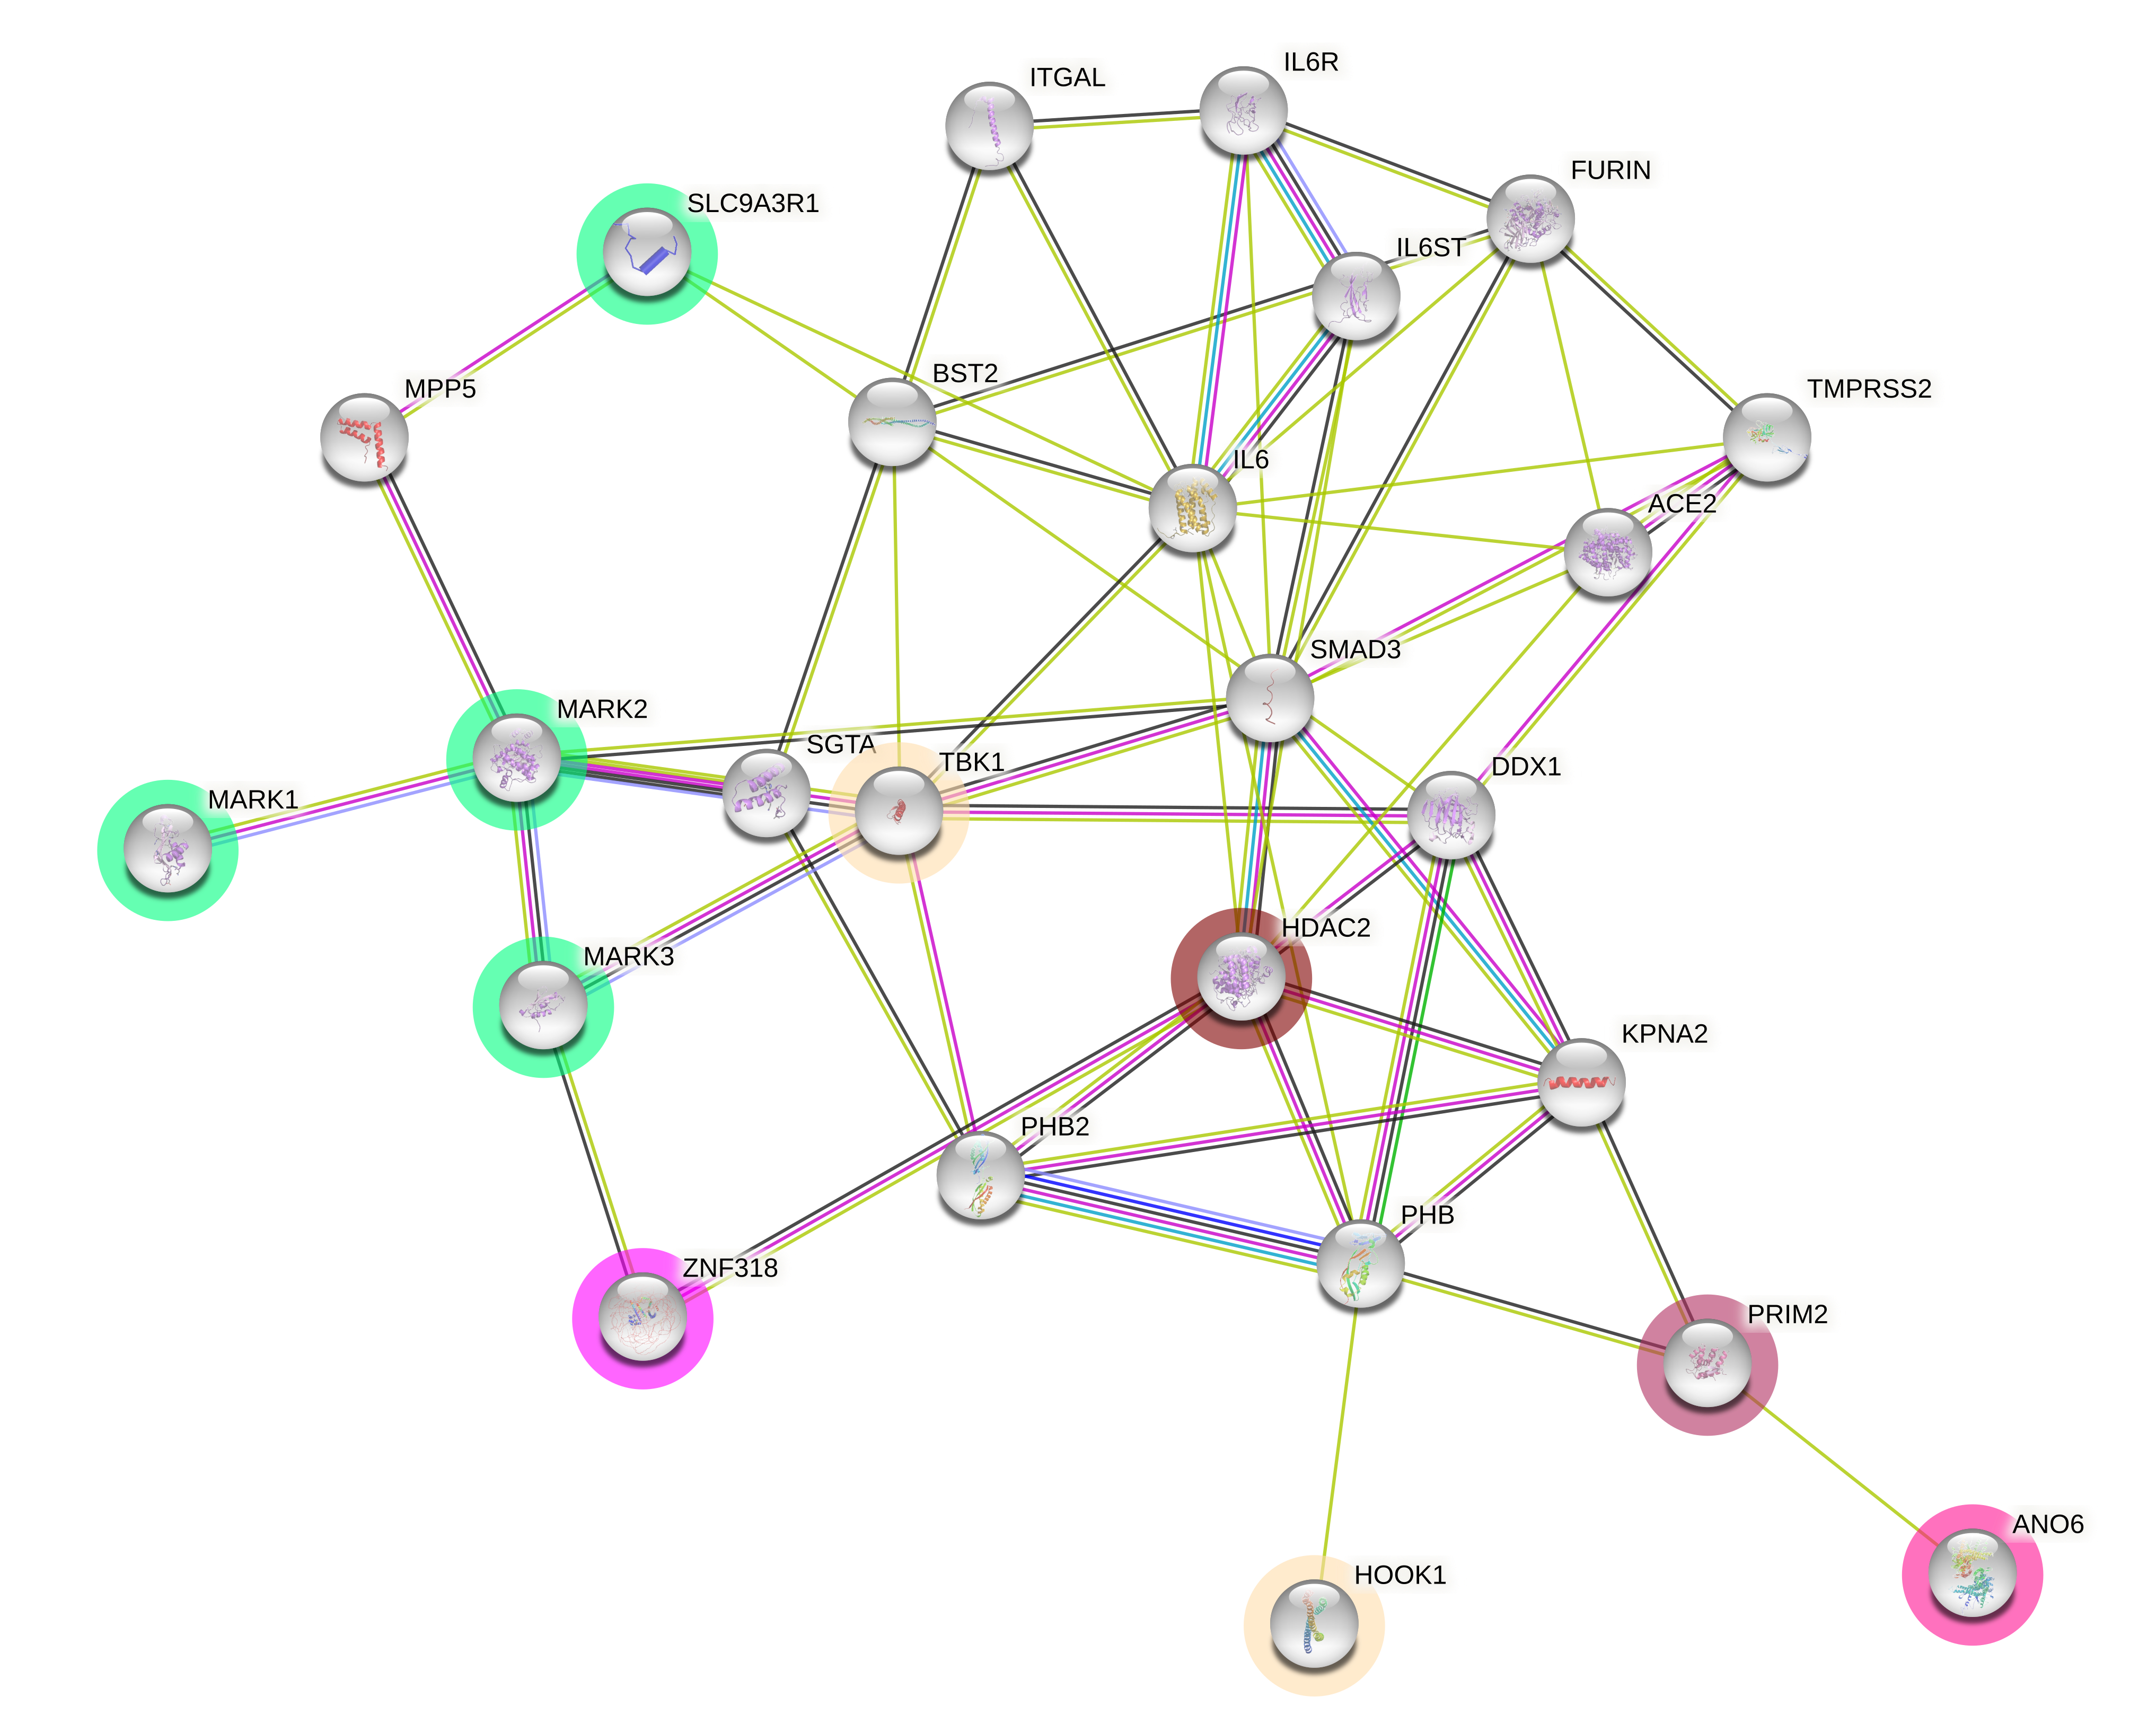
\includegraphics[width=0.9\textwidth]{figures/PPInetSARSCov2BaitProt.png}
		\caption{SARS-CoV-2 protein interaction map}
		\label{fig:ppi_net}
	\end{figure}
	
	\begin{figure}[h!]
		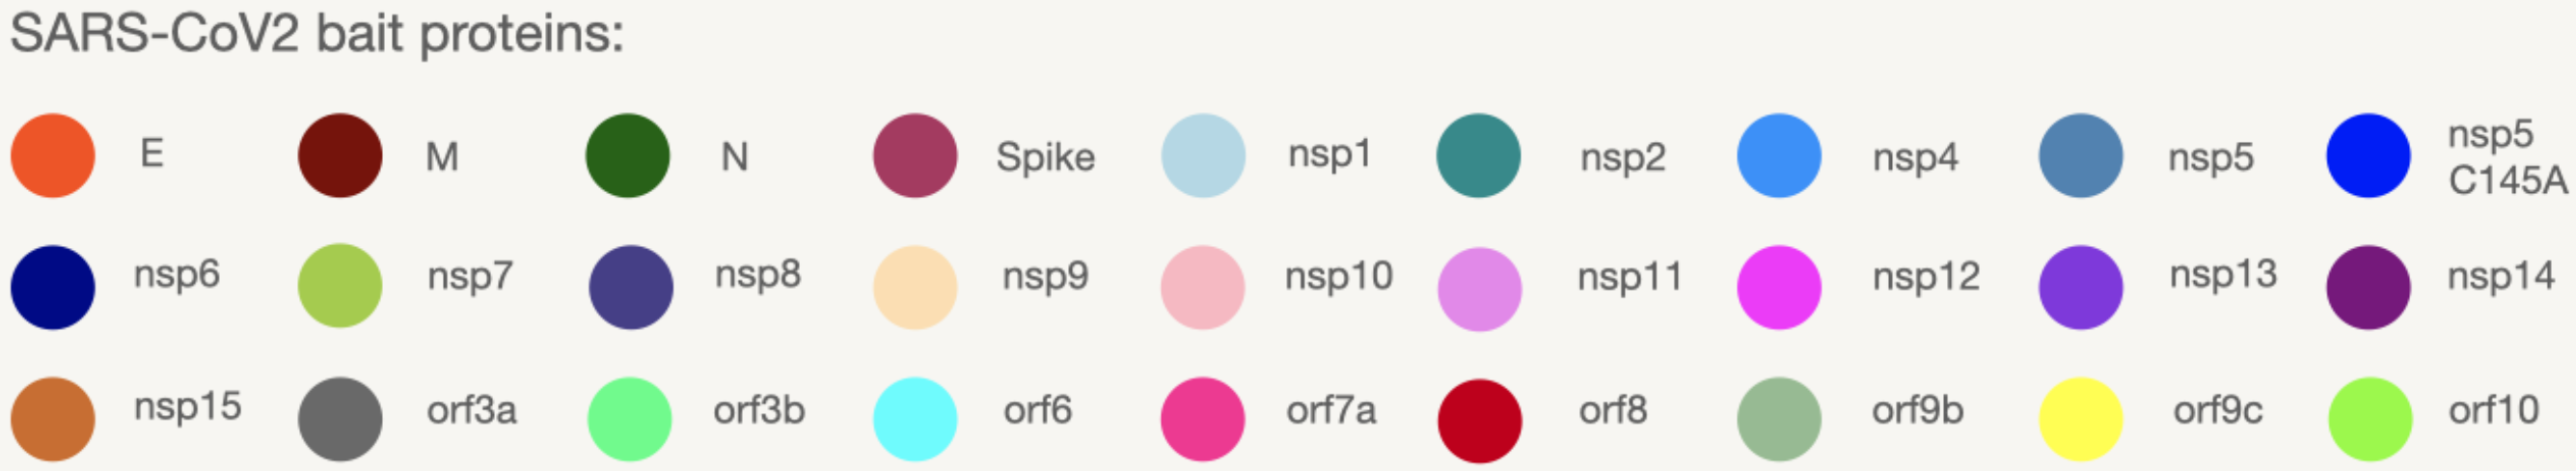
\includegraphics[width=0.9\textwidth]{figures/PPIColourLegend.png}
		\caption{Colour Legend}
		\label{fig:ppi_legend}
	\end{figure}

Se procede a descargar la información casi completa de toda la red (247 de las 332 proteínas)

	\begin{figure}[h!]
		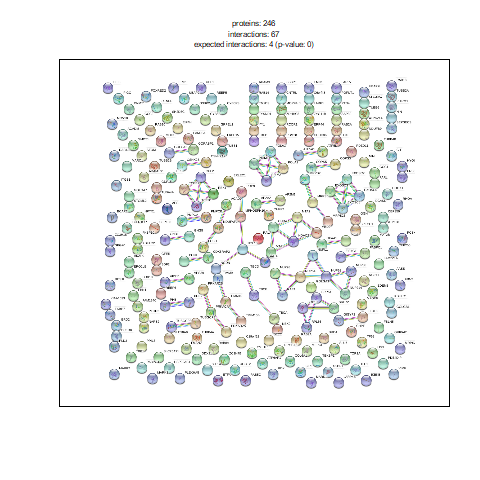
\includegraphics[width=0.9\textwidth]{../results/figuraSTRINGdb.png}
		\caption{SARS-CoV-2 protein interaction map}
		\label{fig:ppi_stringdb}
	\end{figure}
	
	
NOMBRE_DE_LAS_IMÁGENES

figuraLinkcomm.png
figuraSTRINGdb.png
figuraiGraph.png
	
\subsection{Análisis de comorbilidades}